\documentclass[12pt,a4paper]{article}
\usepackage{amsmath, graphicx, hyperref}

\title{Useful Equations}
\author{Ibby EL-Serafy}

\begin{document}
    \pagenumbering{gobble}
    % \maketitle
    \begin{abstract}
        A short intro about this document.
    \end{abstract}

    \tableofcontents

    \section{Introduction}
    
    \begin{figure}
        \centering
        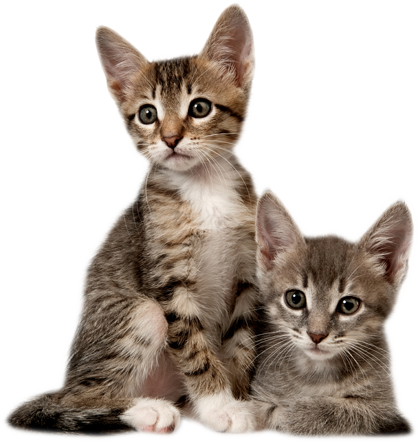
\includegraphics[
            width=0.3\textwidth
        ]{kittens.png}
        % \caption{}
    \end{figure}

    In \ref{sec:maths} we're gonna discuss \ldots

    Apparently `quotes' are ``weird''

    This is a bulleted list:

    \begin{itemize}
        \item Fluids
        \item Electricity
        \item Thermodynamics
    \end{itemize}

    And here's a numbered list:

    \begin{enumerate}
        \item print the pdf
        \item take it with you everywhere you go
    \end{enumerate}

    \section{Includes}
    Hello world!

    \section{Maths \& Equations}
    \label{sec:maths}
    You can do inline equations, for example: $f(x)=A\frac{dy}{dx}+Bx$.
    
You can also have a maths block/section/environment.
    
    \begin{equation*}
        \sum_{i=0}^{\infty}x^i-x^{i-1}
    \end{equation*}

    \subsection{Typesetting maths}
    Here's an aligned equation:
    \begin{align*}
        (x+1)^2(x-4)    &= (x^2+2x+1)(x-4) \\
                        &= x^3+2x^2+x-4x^2-8x-4 \\
                        &= x^3-2x^2-7x-4
    \end{align*}
    Does 3 columns work?
    \begin{align*}
        62 \div 8  &= 7 & \operatorname{rem} 6 \\
        7 \div 8   &= 0 & \operatorname{rem} 7
    \end{align*}
    
\end{document}